\section{Methods and Software}
Monte Carlo physics events and single muons
were simulated using the Simulator for the Linear Collider (SLIC)~\cite{graf2007simulator} program,
which uses the G\textsc{eant}4 toolkit~\cite{agostinelli2003geant4,allison2006geant4}
as the underlying physics engine.
The org.lcsim software framework~\cite{lcsimurl,graf2011org} reconstructs the simulated events
 by first digitizing the simulated tracker hits and then building tracks from these hits,
as described in section~\ref{sec:recon}.
Finally, the Monte Carlo true information and the reconstructed data are 
analyzed and compared to determine each detector's performance.
%The anlaysis step produces ROOT tuples which contain both the Monte Carlo truth and the reconstructed
%data, with which the final analysis steps are completed and plots are produced.
Simulation, reconstruction, and analysis were performed on the grid
using ILCDIRAC version 6.8.28~\cite{1742-6596-513-3-032077}, 
which is an extension of the DIRAC framework~\cite{tsaregorodtsev2008dirac}.
The full software pipeline is illustrated in figure~\ref{fig:software}.
The next section describes the different steps in more detail.
%The simulations were then reconstructed 
%Monte Carlo simulations of physics processes and single muons were performed using 
%-add brief explanation, illustration of simulation, reconstruction, analysis pipeline
%-talk about ILCDIRAC/grid computing
\begin{figure}[b]
\centering
%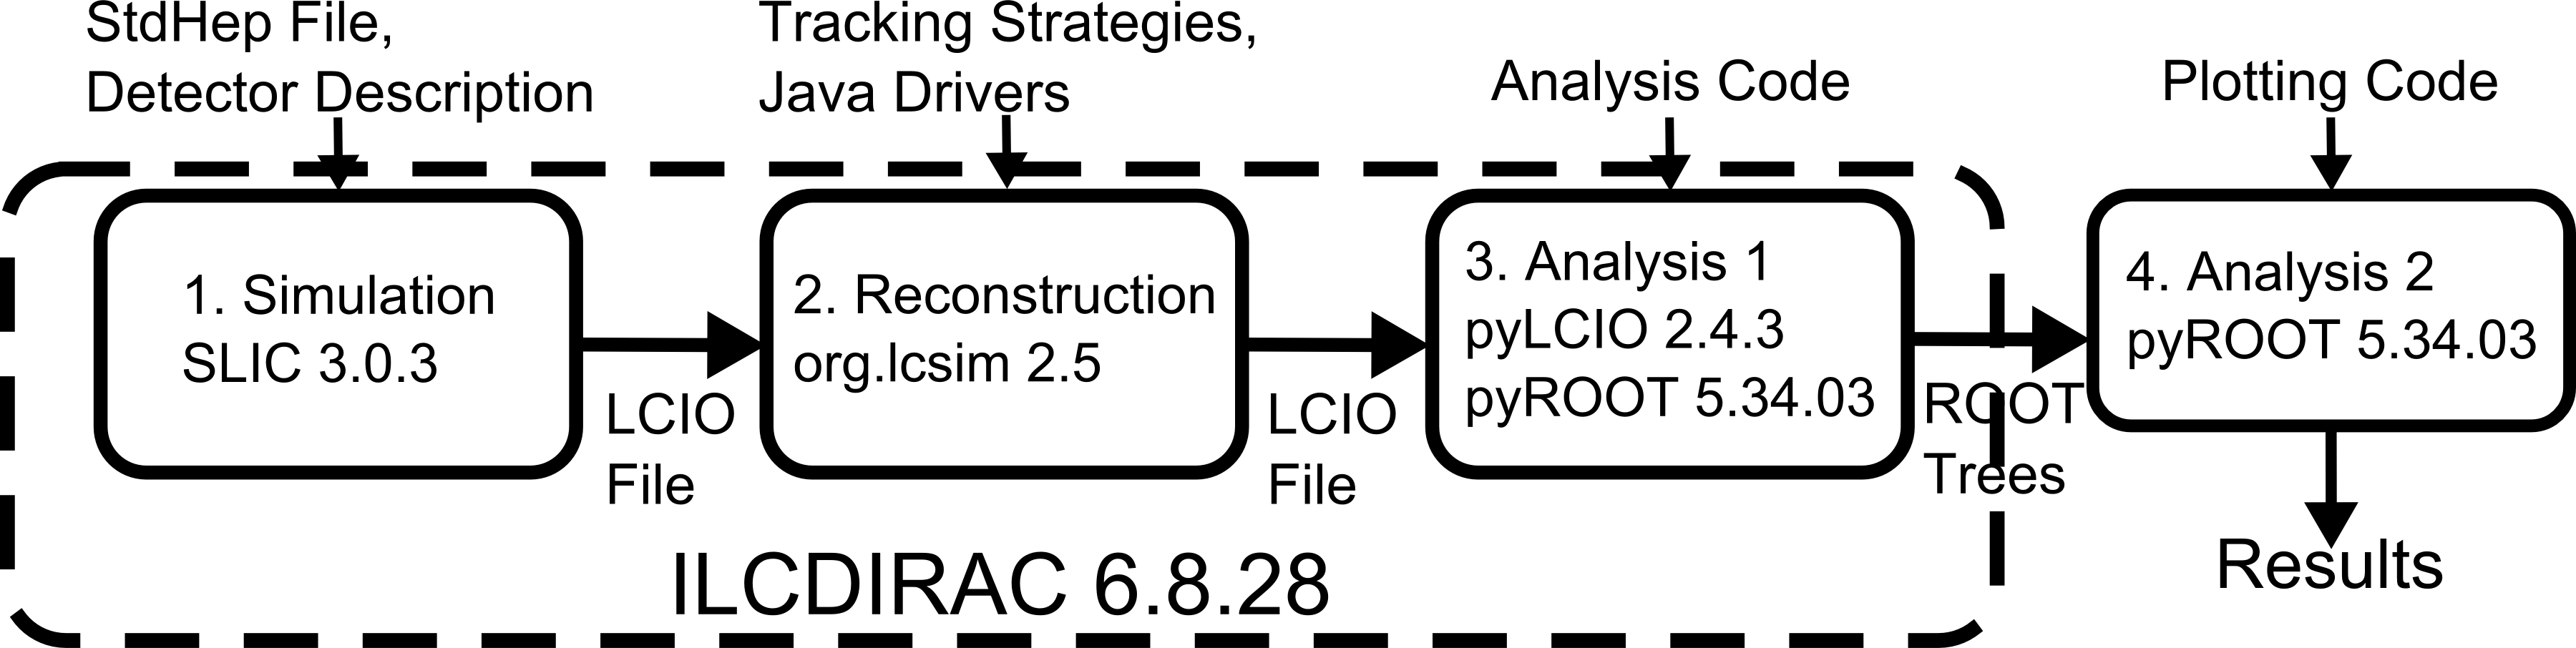
\includegraphics{softwarepipeline1.png}
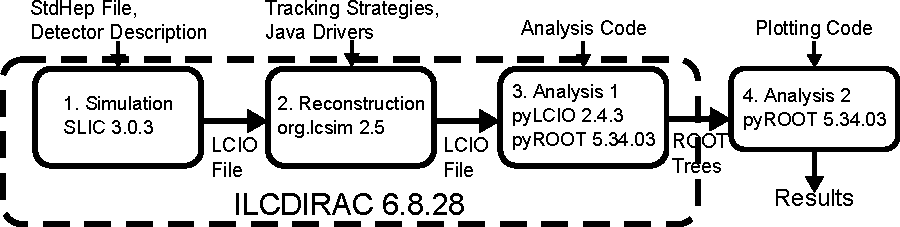
\includegraphics{simReconAnalysisPipeline.pdf}
\caption{The software pipeline for the tracking studies.
%Step one, the simulation step, is described in section~\ref{sec:sim}.
%Step two, the reconstruction step, is described in section~\ref{sec:recon}.
%Steps three and four, the analysis steps, are described in section~\ref{sec:analysis}.
Note that steps one, two, and three are all performed on the grid via ILCDIRAC
version 6.8.28.
The last step is performed locally.}
\label{fig:software}
\end{figure}
\subsection{Detector, Single Particle, and Physics Simulation}
\label{sec:sim}
%Monte Carlo simulations were performed using the Simulator for the Linear Collider (SLIC)~\cite{graf2007simulator} program,
%which uses the G\textsc{eant}4 toolkit~\cite{agostinelli2003geant4,allison2006geant4}and 
SLIC accepts detector geometry definitions in an extensible markup language (XML) format.
The XML description for the modified geometry was made using Sidloi3's XML
description as a template, since both detectors are exactly the same except for the vertex barrel.
SLIC produces simulation files in the Linear Collider Input/Output (LCIO)~\cite{2003physics...6114G} file format.
Simulations utilized SLIC version 3.0.3.

Tracking performance studies were conducted using simulations of single muons,
$\ee \rightarrow \ttbar$ events at $ \sqrt{s} = $ 500 GeV,
and $\ee \rightarrow \ttbar \bbbar$ (hadronic decays only) events at $ \sqrt{s} = $ 1 TeV.
%An input S\textsc{td}H\textsc{ep} file~\cite{stdhep:url} to SLIC gives the
Initial particle four-vectors for the two physics processes were provided as
a S\textsc{td}H\textsc{ep} file~\cite{stdhep:url},
while G\textsc{eant}4's General Particle Source (GPS)
%, also called the `particle gun', 
allows for simulation of muons at user-defined, fixed energies and angles
or user-defined energy and angular distributions.
The physics event samples were generated using the WHIZARD~\cite{kilian2011whizard} event generator,
with hadronization of quarks performed by PYTHIA~\cite{sjostrand2006pythia},
as described in~\cite{Grefe:2014pba,Behnke:2013lya}.
Our studies did not include simulations of beam-induced backgrounds.

G\textsc{eant}4 propagates the simulated particles 
through each layer of the detector discretely, calculating the interaction between each particle and the material of each layer
in order to determine the energy loss and the particle's new position and momentum.
Geant4 knows where to search for material according to the spatial boundaries established by the detector
envelopes, which are shown by white lines in figure~\ref{fig:barrels}.
%This is done discretely for each layer in the detector.
The description of each particle's interaction with the materials in the layers is determined
by a user-defined reference physics list.
The G\textsc{eant}4 QGSP\_BERT physics list~\cite{geant4physlist:url} was used to determine particle interactions with matter, which
 has been shown to agree well with beam tests~\cite{2008arXiv0808.0130P}.
In those parts of a layer which have been designated as `sensitive' (figure~\ref{fig:sidloi3barrel}),
the energy left by a particle is recorded as a `hit'.


\subsection{Tracker Hit Digitization and Event Reconstruction}
\label{sec:recon}
%The digitization and reconstruction of the hits and events generated 
%by SLIC in the detector simulation are
%performed by 
The org.lcsim software framework~\cite{lcsimurl,graf2011org} digitizes the hits
and reconstructs events.
%which are both generated by SLIC during the detector simulation.
Tracker hit digitization, performed by the \textit{SiSim} %\textbf{CITATION?} 
package in org.lcsim,
converts the energy deposits from the simulation step
into digital signals, one per channel~\cite{Grefe:2014pba}. 
%as would be produced from a real detector readout
Charged particle tracks are then reconstructed from these hits using the \textit{SeedTracker}
algorithm %\textbf{CITATION?}
 in org.lcsim, which finds tracks  according to user-generated,
detector-specific tracking strategies~\cite{Grefe:2014pba}.
(See section~\ref{sec:trackingstrategies}.)
The output LCIO file from org.lcsim contains the reconstructed
tracks and their parameters, the Monte Carlo true parameters for each simulated
particle, and relational tables between each reconstructed tracker hit
and the Monte Carlo particle associated with it, which allows the analysis
of tracking performance.
Our studies used org.lcsim 2.5.

The segmentation of the various tracking layers is implemented after the simulation and
during the reconstruction step using Java drivers~\cite{Grefe:2014pba}.
For pixel sensors, both the sensor and readout pitches are set to $20~\mu m$ in $x$ and $y$.
%which are local dimensions for each module and run parallel to the plane of the sensor.
Pixellated segmentation is used in the vertex barrels and disks.
For strip sensors, which run parallel to the global $z$-axis, 
the sensor pitch is set to $25~\mu m$ and the readout pitch is set to $50~\mu m$.
Thus, every other strip is directly read out.
%Those strips which are not directly read out are indirectly read out via
The intermediate strip is coupled
capacitively to the readout strips~\cite{krammer1997signal}.
%No additional pitch value needs to be defined because
%the length of the strip sensors equals the length of their subdetector modules.
The segmentation along the section is 10~cm, the length of the sensor.
Strip segmentation is used in the tracker barrels and disks.
A nearest neighbor algorithm clusters digitized hits
that are near each other~\cite{Grefe:2014pba}.
These clusters of hits form the tracking hits which
the \textit{SeedTracker} algorithm uses to reconstruct tracks.
In the LCIO data model, five unique geometric parameters
define a helix~\cite{kramer2006track}.
Using the L3 convention~\cite{alcaraz1995helicoidal},
these parameters are $d_{0}$, $\kappa$, $\phi_{0}$, $\tan{\lambda}$, and $z_{0}$,
 illustrated in figure~\ref{fig:helix}.
From these helix parameters, the track's physical quantities
may be determined according to the following equations~\cite{Grefe:2014pba}.
%\begin{tabularx}{\textwidth}{cc}
%\begin{equation}
%\begin{aligned}
%\begin{split}
\begin{flalign}
\nonumber
&p_{T} = kB/|\kappa|,\mbox{ }k = 0.003 \mbox{ GeV T$^{-1}$ mm$^{-1}$} \\\nonumber
&p_{x} = p_{T}\cos{\phi_{0}}\\\nonumber
&p_{y} = p_{T}\sin{\phi_{0}}\\\nonumber
&p_{z} = p_{T}\tan{\lambda}\\\nonumber
&p = p_{T}/\cos{\lambda}\\\nonumber
&q = \kappa/|\kappa|
\label{eq:helixparam}
\end{flalign}
%\end{split}
%\end{aligned}
%\end{equation}
%& 
%\end{tabularx}
For a discussion of the uncertainty in the track parameters and their propagation, see~\cite{Grefe:2014pba}.
\begin{figure}[t]
\centering
%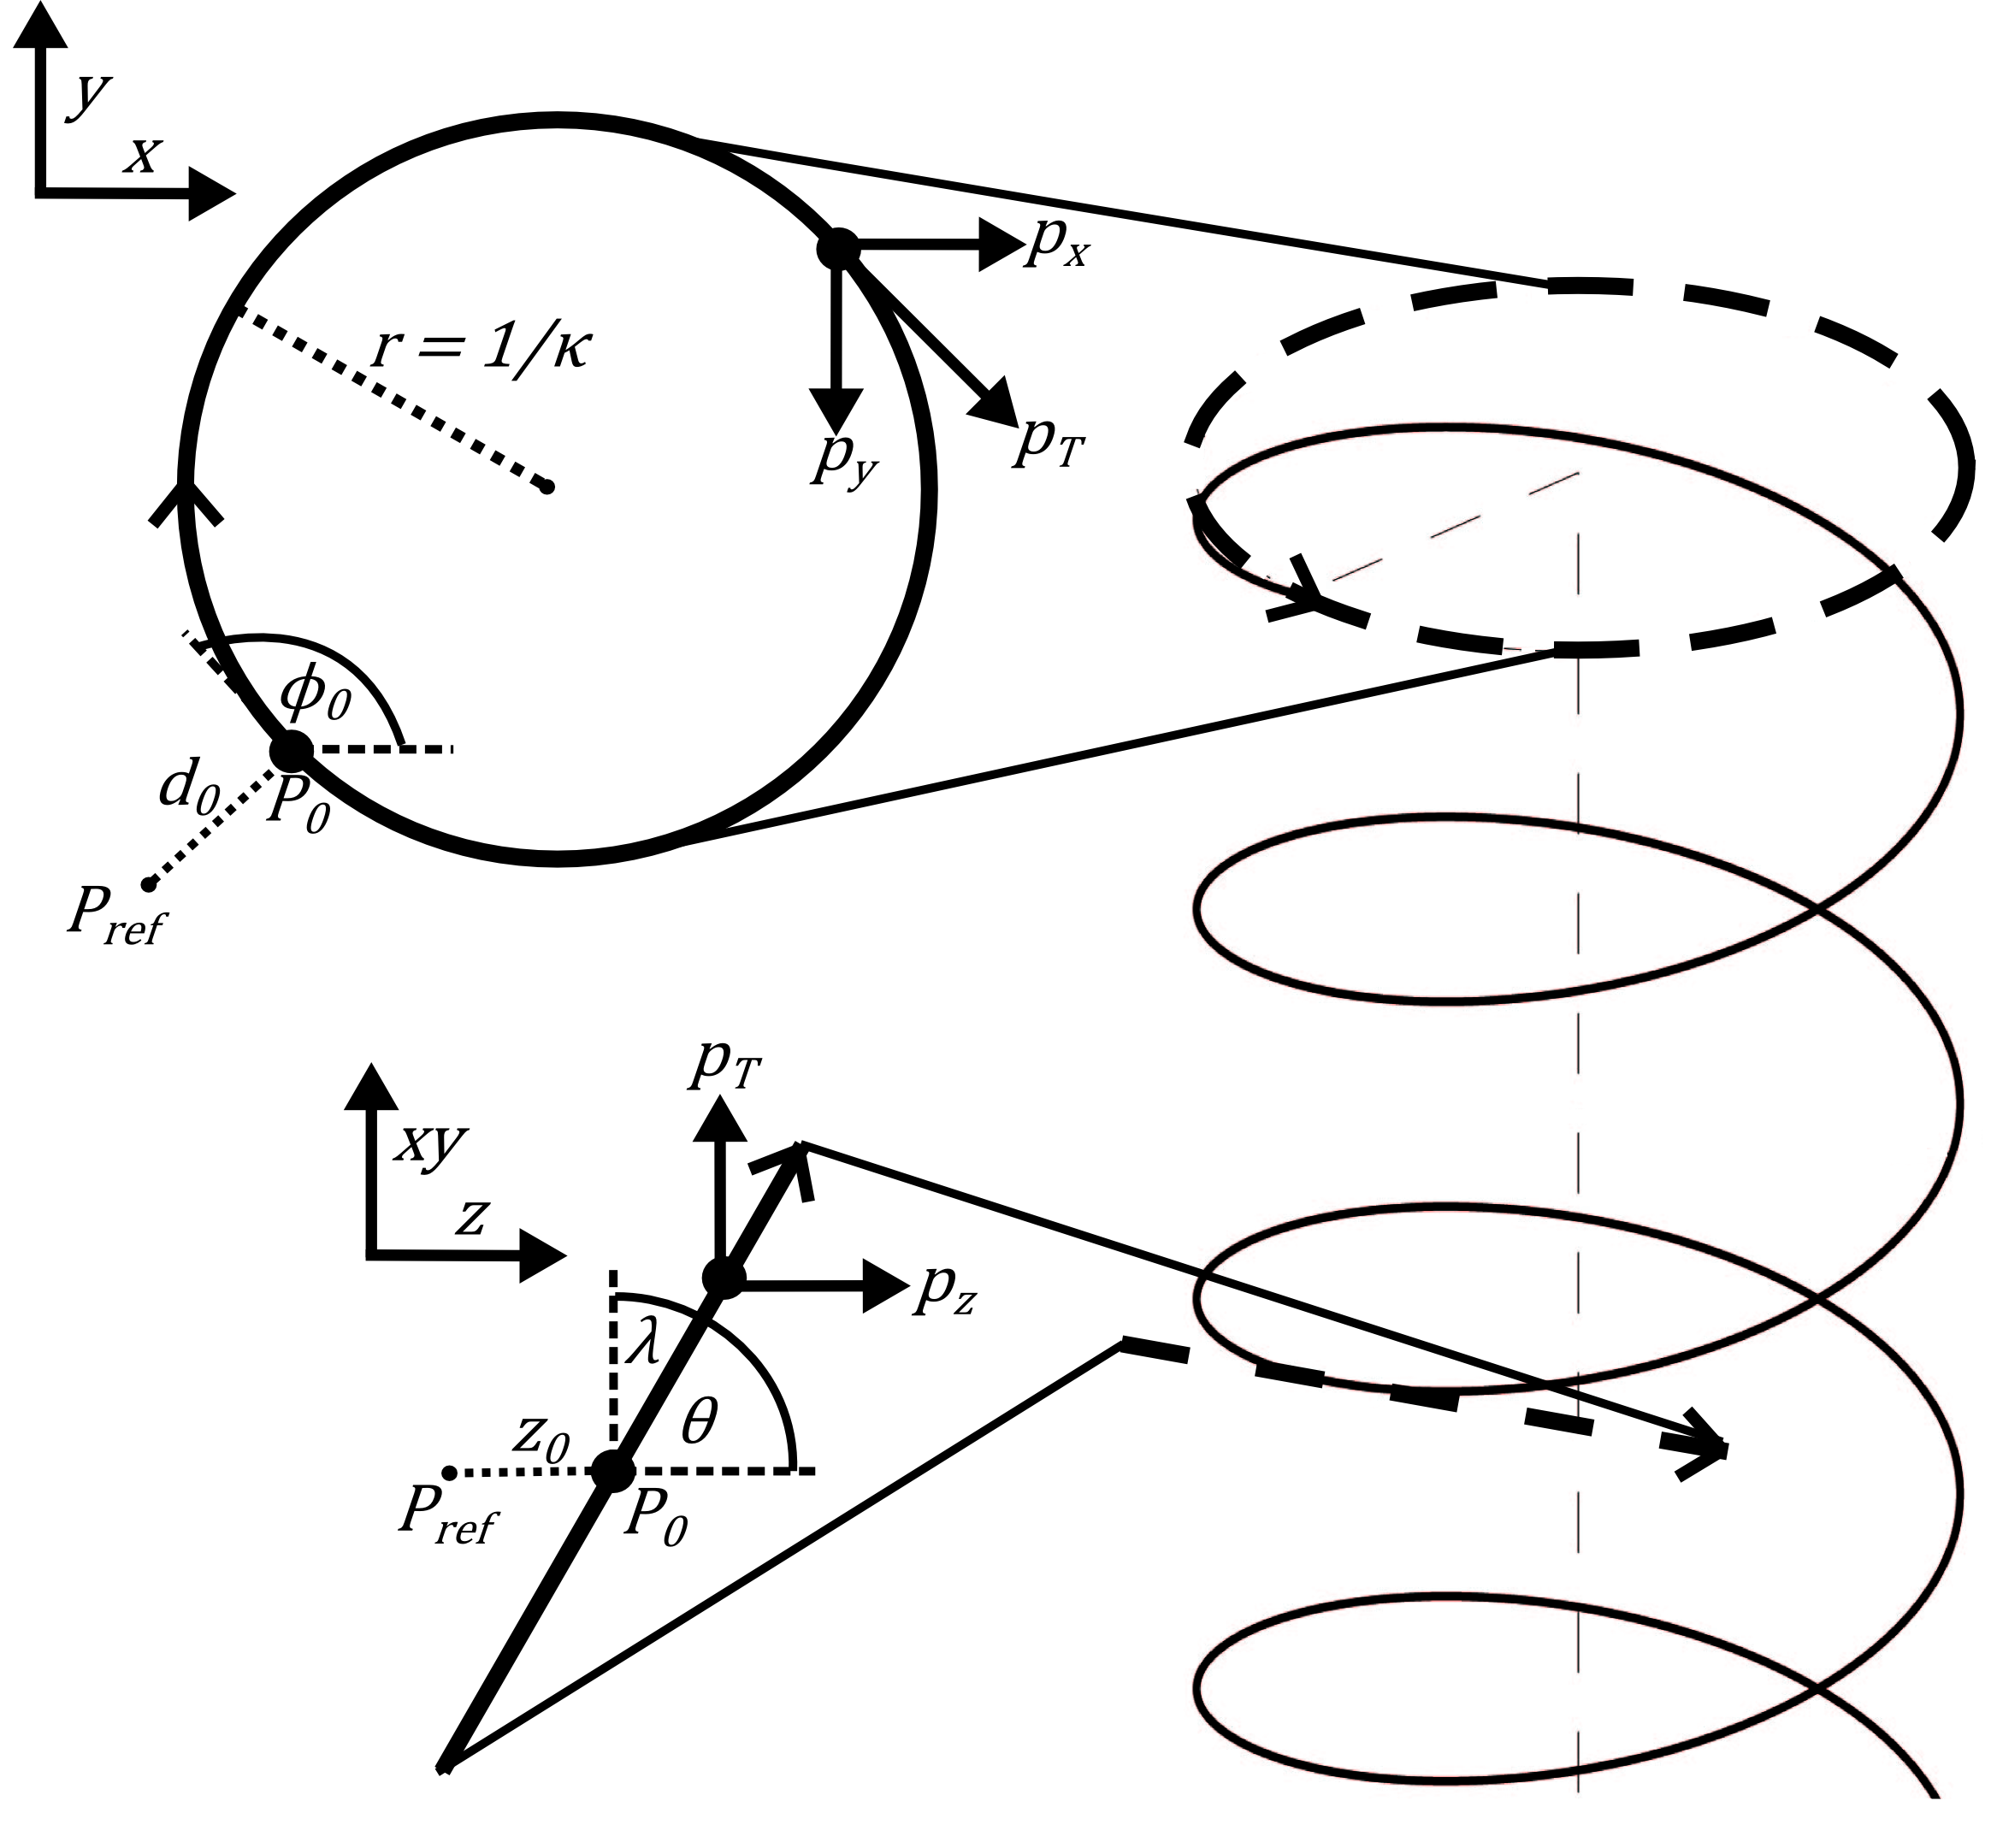
\includegraphics{helixDrawing5.png}
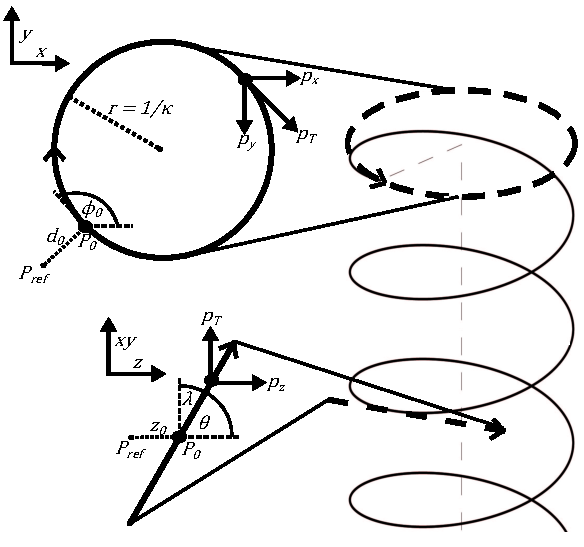
\includegraphics{helixDrawing3.pdf}
\caption{LCIO track parameter definition.
Parameters are defined with respect to $P_{ref}$, which we place
for convenience at the origin (0,0,0).
Point $P_{0}$, with coordinates ($x_{0}$,$y_{0}$,$z_{0}$), marks the starting point of the helix,
which is the track's $xy$ projection's closest point
of approach to $P_{ref}$. The $xy$ 
impact parameter $d_{0}$ is given by $d_{0} = \sqrt{x_{0}^{2}+y_{0}^{2}}$.
From the track parameters,
physical parameters may be calculated via equations~\ref{eq:helixparam}.}
\label{fig:helix}
\end{figure}

\subsubsection{Tracking Strategies}
\label{sec:trackingstrategies}
The \textit{SeedTracker} algorithm relies on a group of tracking
strategies to reconstruct tracks.
Each tracking strategy is a set of tracker layers %within the detector 
from which the algorithm must use tracker hits to
 produce the reconstructed helical tracks of charged particles.
%org.lcsim accepts tracking strategies in an XML format.
Each reconstructed track produced by a given strategy must satisfy
the track parameter and helix fit requirements listed in table~\ref{tab:stratCuts}.
Each strategy assigns one of three roles to each tracking layer: seeding,
confirming, and extending.
In any given strategy, there are 3 seed layers, 1 confirm layer,
and any additional number of extend layers.
All combinations of hits from the 3 seed layers form the initial 
set of possible tracks.
An initial helix fit to each candidate determines
the track parameters.
Then, each candidate is tested with each hit in the confirm layer
for another helix fit and only those hits are kept whose 
addition to the fit keeps $\chi^{2} < \chi^{2}_{max}$,
one of the cuts listed in table~\ref{tab:stratCuts}.
Only those hits in the confirm layer whose position in $\phi$ and $z$ are
consistent with a given candidate's initial parameters are tested.
Multiple confirmed seeds from a single possible track are possible.
Finally, each seed is extended layer by layer using the hits
in the extend layers, so long as the various cuts specified in table~\ref{tab:stratCuts}
are still met.
As with the confirm layer, only hits with $\phi$ and $x$ positions plausible for
the given track are tested.
Once there are not enough layers remaining for a seed track to satisfy $N_{min}$,
that track is discarded.
If the track being reconstructed shares more than one hit in common with a previously
reconstructed track, the track with more hits is kept or, in the case
of tracks with equal hit numbers, the track with lowest $\chi^{2}$.
For details concerning the helix fitting and accounting of multiple scattering,
see~\cite{Grefe:2014pba}.

\begin{table}[t]
\begin{center}
\begin{small}
	\begin{tabular}{c||cc}
	\textbf{Track, Fit Parameters} & \textbf{Barrel Only Strategy} & \textbf{All Other Strategies} \\
	\hline \hline
	$ N_{min} $ & 6 & 7 \\
	$ p_{T,min} $ & 0.2 & 0.2 \\
	$ d_{0,max} $ & 5.0 & 10.0 \\
	$ z_{0,max} $ & 10.0 & 10.0 \\
	$ \chi^{2}_{max} $ & 10.0 & 50.0 \\
	\end{tabular}
\caption{Cuts on several reconstructed track parameters and the $\chi^{2}$ of the helix fit.
The cuts are passed to the tracking strategies to define acceptable reconstructed tracks.
$N_{min}$ refers to the minimum number of hits required for a reconstructed track.
Refer to figure~\ref{fig:helix} to see the track parameters $p_{T}$, $d_{0}$, and $z_{0}$ illustrated.
%$\chi^{2}$ is the parameter which the helical fitting algorithm aims to minimize.
The barrel only strategy is designed for finding low $p_{T}$ tracks at high polar angles
whose radius of curvature is lower than the seventh tracker layer.
It requires only six hits but uses a more strict $\chi^{2}$ cut
than that used for all other strategies.
The effect of varying the $N_{min}$ and $\chi^{2}$ cut on tracking efficiency
is shown in~\cite{Grefe:2014pba}}
\label{tab:stratCuts}
\end{small}
\end{center}
\end{table}

Tracking strategies may be produced manually
by creating lists of seed, confirm, and extend layers
with which one would like reconstruct tracks.
However, the preferable manner for making
strategies involves generating the strategies
via an org.lcsim software tool and a sample physics process
with the required angular and energy distributions~\cite{Grefe:2014pba}.
Ideally, the sample physics process used to build
the strategies should densely
populate the phase space.
For our tracking studies,
two sets of strategies were generated, one using
500 $\ee \rightarrow \ttbar$ events at $ \sqrt{s} = $ 500 GeV
and another using 500 $\ee \rightarrow \ttbar \bbbar$ (hadronic decays only) events at $ \sqrt{s} = $ 1 TeV.
The $\ttbar$-generated strategies were used to reconstruct single muon tracks and $\ttbar$ events.
The $\ttbar \bbbar$-generated strategies were used to reconstruct $\ttbar \bbbar$ events.
%500 $\ee \rightarrow \ttbar$ events at $ \sqrt{s} = $ 500 GeV generated the 
%strategies for reconstructing single muon tracks and $\ee \rightarrow \ttbar$ events at $ \sqrt{s} = $ 500 GeV.
%500 $\ee \rightarrow \ttbar \bbbar$ (hadronic decays only) events at $ \sqrt{s} = $ 1 TeV generated the
%strategies for reconstructing $\ee \rightarrow \ttbar \bbbar$ (hadronic decays only) events at $ \sqrt{s} = $ 1 TeV.

\subsection{Analysis}
\label{sec:analysis}
The output LCIO files from org.lcsim were analyzed
using Python code.
 ROOT trees were generated by linking the pyLCIO and pyROOT bindings
to the respective LCIO and ROOT C++ libraries.
Each ROOT tree contains the helix and physical parameters
for both the Monte Carlo particles and 
the reconstructed tracks. %generated by org.lcsim.
The trees also map tracks
to the Monte Carlo particles,
allowing for the comparison between the Monte Carlo
truth of helix and physical parameters with their reconstructed values.
Such comparisons enable study of
 the tracking performance of each detector.% is studied.
The ROOT trees, which are produced on the grid via ILCDIRAC, are then
downloaded locally and further analyzed to produce the final results.
%These results include tracking efficiencies vs. $p_{T}$, $\theta$, and number of hits;
%fake rates on tracks vs. $p_{T}$ and $\theta$;
%$\sigma(d_{0})$ and $\sigma(z_{0})$ vs. $\theta$ (impact parameter resolutions);
%and $\sigma(p_{T})/p_{T}^{2}$ vs. $p$ (transverse momentum resolution).

%For analysis purposes,
%stricter definitions for findable Monte Carlo
%particleshose Monte Carlo particles which were considered `findable' by the detect


%%%%%%%%% CITATION EXAMPLE
%Recently the dominant ultrasoft NNLL corrections have been 
%completed~\cite{Hoang:2006ht,Pineda:2011aw,Hoang:2011gy}. The accuracy
%in this calculation is illustrated in Fig.~\ref{fig:tthresh-hs}.
\iffalse
%%%%%%%%%%%%%%%%%%%%%%%%%%%% FIGURE EXAMPLE
\begin{figure}
\centering
%\includegraphics[width=0.7\columnwidth]{ttthresh_hs.pdf}
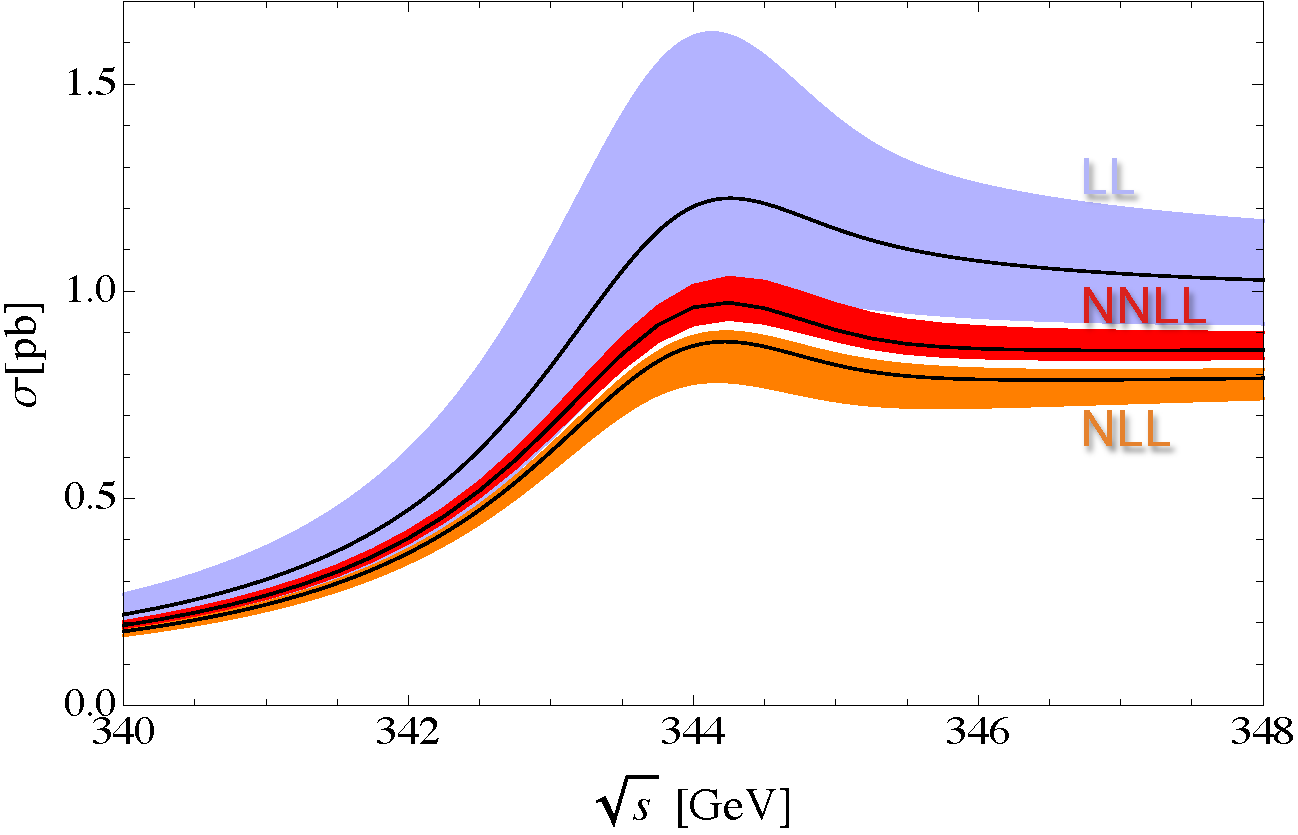
\includegraphics[width=0.7\columnwidth]{TotCrossCombined.pdf}
\caption{
%Accuracy on the prediction of the top pair production 
%cross section at the $t\bar{t}$~threshold at the ILC as achieved by 
%recent calculations of QCD corrections (NNLL). For further explanations 
%see text. The figure has been taken from~\cite{bib:topws-ms}.
Bands show the theoretical QCD uncertainties of the prediction of the top pair production cross section at the $t\bar t$ threshold
   at the ILC as achieved by recent renormalization-group-improved QCD calculations~\cite{Hoang:2013uda}. Their analysis estimated 
   the theoretical uncertainty in the total cross section as $d\sigma_{t\bar t}/\sigma_{t\bar t}\pm 5\%$. For further explanation see text.
}
\label{fig:tthresh-hs}
\end{figure}
%%%%%%%%%%%%%%%%%%%%%%%%%%%%%%%


%%%%%%%%%%%%%%%%%%%%%%%%%%%%%%%%%%%%%%%%%%%%%%%%%%%%%
\begin{figure}
\centering
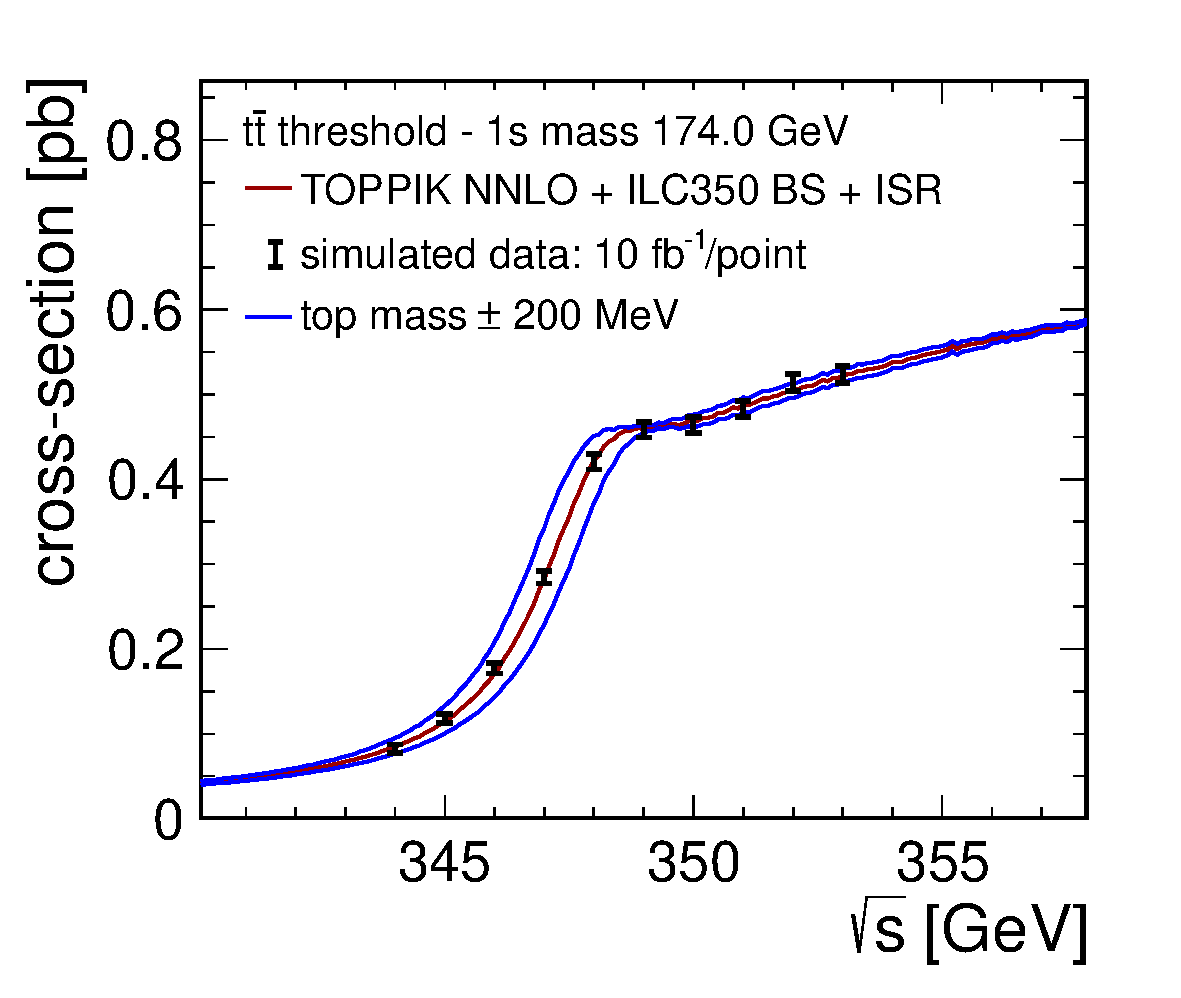
\includegraphics[width=0.50\columnwidth]{ILC_TopThreshold.pdf}
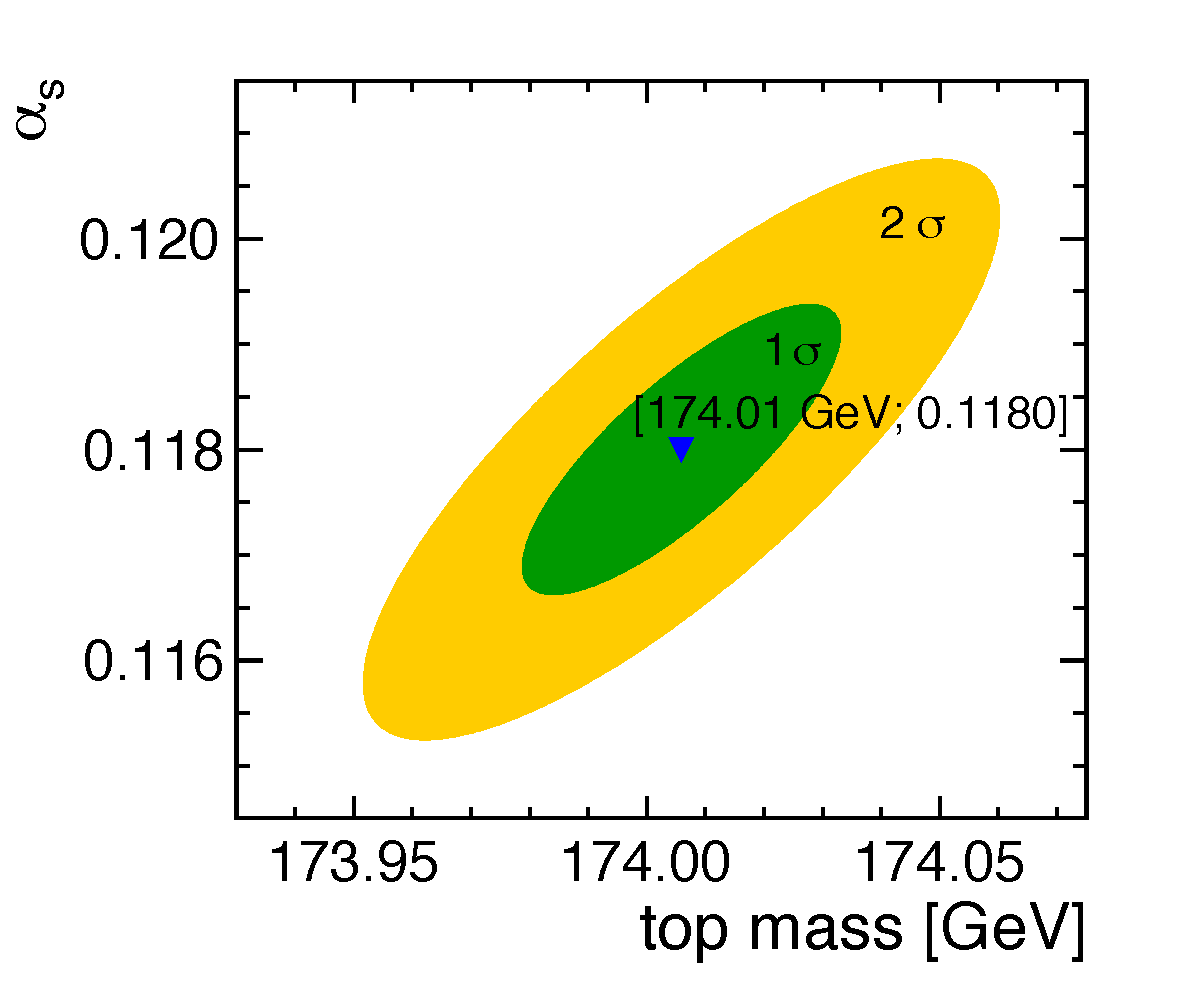
\includegraphics[width=0.40\columnwidth]{contours-10-ilc.pdf}
\caption{Illustration of a $t$~quark threshold measurement at the ILC. 
In the simulation, the $t$~quark mass has been 
chosen to be 174.~GeV.  The blue lines show the effect of varying this 
mass by 200~MeV. The study is based on full detector simulation and takes 
initial state radiation (ISR) and beamstrahlung (BS) and other relevant 
machine effects into account: (left) the simulated threshold scan.  (right) 
error ellipse for the determination of $m_t$ and $\alpha_s$. The figure is
 taken from~\cite{Seidel:2013sqa}.}
\label{fig:ttthresh-scan}
\end{figure}
%%%%%%%%%%%%%%%%%%%%%%%%%%%%%%%%%%%%%%%%%%%%%%%%%%%%%%%%%%%%%%%% 
\fi
\iffalse
\begin{table}
\centering
\begin{tabular}{|ccc|}
\hline
\multicolumn{3}{|c|}{1S top mass and $\alpha_s$ combined 2D fit}\\
\hline
Error type & ILC & CLIC \\
\hline
 $m_t$ stat. error &  27~MeV & 34~MeV\\
 $m_t$ theory syst. (1\%/3\%) &  5~MeV / 9~MeV & 5~MeV / 8~MeV\\
 $\alpha_s$ stat. error & 0.0008 & 0.0009\\
 $\alpha_s$ theory syst. (1\%/3\%) & 0.0007 / 0.0022 & 0.0008 / 0.0022 \\
\hline
\end{tabular}

\caption{Results summary for the 2D simultaneous top mass and $\alpha_s$ determination with a threshold scan at CLIC and ILC for 10 points with a total integrated luminosity of 100\,fb$^{-1}$~\cite{Seidel:2013sqa}. \label{tab:ThresholdResults}}
%Event selection and background rejection from CLIC\_ILD is used.\label{tab:ThresholdResultsILC}}
\end{table}
\fi